\documentclass[../full_thesis/full_thesis.tex]{subfiles}

% Default image directory
\newcommand{\thisdir}{../detecting_cgw}
\graphicspath{{\thisdir/img/}}

\begin{document}

Timing variations, in the form of glitches or timing-noise, may pose a serios
risk to efforts to discover continuous GWs from neutron stars. This is because
searches rely on \emph{matched-filtering} which searches the data using a
template; if the template and signal don't match, due to timing variations in
the signal, the template may be unable to detect the signal. In this section
we will give a general introduction to detection methods used in GW data
analysis, explain why timing variations pose a risk, and introduce some simple
calculations. The details of estimating the risk for glitches and timing noise
will be covered in Chapter~\ref{sec: glitches in cgw} and Chapter~\ref{sec:
timing noise in cgw} respectively.

\section{Introduction}
Rotating neutron stars capable of supporting non-axisymmetric mass
distributions will emit continuous gravitational
waves\footnote{Note that in general ``continuous waves'' can
    refer to any quasi-monochromatic long-lasting gravitational-wave
        signals, such as emitted by binaries of white dwarfs, neutron
        stars or black holes, which would be detectable by LISA or pulsar
        timing arrays. Here we refer to CWs exclusively in the context of
        spinning nonaxisymmetric neutron stars as relevant to ground-based
        detectors.}
(CWs) due to their
time-varying quadrupole moments. These may be detectable by next-generation ground-based detectors. The emitted
signals can persist for longer than
typical search durations, but are weak in amplitude, making them difficult to detect
in the noise of the detector.

To find a signal, CW searches use matched
filtering techniques such as the $\mathcal{F}$-statistic \citep{Jaranowski1998}
which compare the output of the detector with a template.  These techniques are
powerful provided that the signal and template remain coherent for the duration
of the observation. If the signal can be perfectly matched by a template then
the signal to noise ratio, used to quantify the detection likelihood, scales as
$\rho^{2} \propto \To$ (e.g.\ see~\citep{Prix2009}). This suggests searching
over longer observations increases the chances of making a detection.

The templates must model the monotonic spin-down of the source due to the
electromagnetic (EM) and gravitational torque; this is done by Taylor expanding
the phase:
\begin{equation}
\phi(t) = \phi_{0} + 2\pi\left(\f_{0} (t - t_{0}) +
          \frac{\fdot_{0}}{2!} (t - t_{0})^{2}
           %+ \frac{\fddot}{3!} (t - t_{i})^{3}
           \right)
           + \ldots
           \,,
\label{eqn: Taylor}
\end{equation}
where $t_{0}$ is the reference time at which the pulsar frequency, and
spin-down parameters $[\phi_{0}, \f_{0}, \fdot_{0}, \ldots]$ are defined. Note
that all times refer to the solar system barycentre and we assume the
timing model has already correctly accounted for the dispersion measure, proper motion
and other parameters as discussed in \citet{Edwards2006}.
Pulsar astronomers fit this model to observed time of arrivals (TOAs). If the
best fit model is accurate enough to track the pulsar to within a single
rotation the resulting timing solution is described as \emph{phase-connected}.
Often such solutions are capable of tracking the pulsar over durations greater
than  a year \citep{Lyne2012book}.  For gravitational-wave searches, this level of accuracy
motivates the use of the same Taylor expansion phase models to account for the
spin-down.  Pulsar observers measure the frequency $\f_{0}^{EM}$ and higher
order coefficients describing the rotation of the pulsar itself. In this
work generally we will consider only searches for
emission from non-axisymmetric neutron stars at
$\f_{0}^{CW}=2\f_{0}^{EM}$~\citep{Shapiro83}; from hereon all frequencies
and spin-downs refer to the pulsars CW emission.


\section{Introduction to the mismatch}
\label{sec: introduction to the mismatch}
While Taylor expansion models are on average reliable enough to track the
spin-down, pulsars do show timing variations either in the form of glitches,
occasional sudden increases in the rotation frequency, or continuous
low-frequency variations known as \emph{timing noise}. To quantify the effect
these variation will cause, we will use the \emph{mismatch} which is the loss
of signal to noise ratio due to the imperfect matching the template and the
signal. The mismatch is non-zero whenever the signal and template are not
perfectly matched. Even if the signal does not contain any timing variations a
mismatch can occur when the template, chosen from a finite grid of points in
parameter space, does not share exactly the same parameters as the signal. This
problem has been studied in detail since finite computing resources limit the
number of templates which can be used in a search and ensure that any
prospective search must have some level of mismatch. In the this section
we introduce the tools which have been developed to understand this problem. We
will return to the problem of timing variations later on in this chapter.



\subsection{Defining the mismatch}

We begin by assuming that the gravitational-wave detector strain data contains
a periodic CW signal with phase $\PhiS(t; \ls^{\alpha})$, where $\ls^{\alpha}$
is a vector of the signal parameters. A fully-coherent search consists of
applying a matched-filtering algorithm over a coherence time $\Tcoh$ to search
the data using a \emph{template}; let us then denote the phase evolution of the
template as $\PhiT(t; \lt^{\alpha})$, such that $\lt^{\alpha}$ is a vector of
the template parameters.

Defining the phase-difference between the signal and the template as
\begin{align}
\Delta\Phi(t; \lt^{\alpha}, \ls^{\alpha}) = \PhiS(t; \ls^{\alpha}) - \PhiT(t; \lt^{\alpha}),
\label{eqn: phase diff}
\end{align}
then, following the work of \citet{Prix2005} and neglecting amplitude modulations
in the signal, we can define the matched-filtering amplitude
\begin{equation}
X = \frac{1}{\Tcoh}\int_{\Tcoh}e^{i\Delta\Phi} dt.
\label{eqn: matched filtering amplitude}
\end{equation}
Defining $\rhotilde$ as the signal to noise ratio (SNR) measured in a fully-coherent
search, then the matched-filtering amplitude defines the loss of SNR incurred
due to the non-zero phase difference with respect to a perfectly matched signal
with SNR $\rhotilde_{0}$ such that
\begin{align}
\rhotilde = |X|\rhotilde_{0}.
\end{align}
An simple dimensionless measure of the loss of SNR is found by rearranging
and defining the fully-coherent \emph{mismatch} as
\begin{equation}
\mutilde(\ls^{\alpha}, \lt^{\alpha}) = 1 - |X(\ls^{\alpha}, \lt^{\alpha})|^{2},
\label{eqn: full mismatch}
\end{equation}
such that
\begin{equation}
\mutilde = \frac{\rhotilde_{\mathrm{pm}}^{2} - \rhotilde^{2}}
                {\rhotilde^{2}_{\mathrm{pm}}}.
\label{eqn: numeric mismatch}
\end{equation}

\subsection{Interpreting the mismatch}
In this work we will quantify the effect of glitches by the mismatch. However,
it may useful to interpret a mismatch in the following way. For a perfectly
matched continuous GW signal it can be shown \citep{Jaranowski1998} that the SNR scales as
\begin{equation}
\rho_{0} \propto \frac{h_{0}}{\sqrt{\textrm{S}_{\textrm{n}}}}
                               \sqrt{\Tobs \mathcal{N}}
\end{equation}
where $h_{0}$ is the strain-amplitude from an optimally oriented source with
respect to the detector, $\sqrt{\textrm{S}_{\textrm{n}}}$ measured the noise
in the detector and $\mathcal{N}$ is the number of detectors.

Combining this equation with Eqn.~\eqref{eqn: numeric mismatch}, the SNR of a signal
with mismatch $\mutilde$ scales as
\begin{equation}
\rho \propto \sqrt{1-\mutilde} \frac{h_{0}}{\sqrt{\textrm{S}_{\textrm{n}}}}
                               \sqrt{\Tobs \mathcal{N}},
\end{equation}
which is to say it reduces the sensitivity by a factor~$\sqrt{1-\mutilde}$.



\subsection{Taylor expansion signals and templates}
So far we have not yet defined a phase evolution model for either the signal or the template.
The signal phase $\PhiS(t; \ls^{\alpha})$ will depend on the GW production mechanism,
but assuming the signal is generated by the canonical non-axisymmetric distortion,
the GW signal will be produced at twice the rotation frequency and spin-down
with twice the rotational spin-down rate. From the success of pulsar astronomy,
we know that the phase evolution of the rotation can be modelled by a Taylor
expansion, typically up to the first order in frequency derivative. Therefore,
we can begin by modelling the GW phase evolution using a Taylor expansion
\begin{equation}
\PhiS (t, \ls^{\alpha}) = \phiS + 2\pi \left(\nuS (t - \tref)
+ \frac{\nudotS}{2}(t - \tref)^{2} \right),
\label{eqn: Taylor lambda signal}
\end{equation}
such that $\ls^{\alpha} = [\phiS, \nuS, \nudotS]$. In principle, we can include
higher order terms, but for this work we truncate at the first
derivative of the frequency.

For blind searches, where we have no hints about the phase evolution,
typical continuous GW searches assume that the GW signal is a Taylor expansion and
search for it using Taylor expansion template. Defining $\lt^{\alpha} = [\phiT,
\nuT, \nudotT]$ as the Taylor expansion
template parameters, Eqn.~\eqref{eqn: phase diff}, the phase difference, is
\begin{align}
\Delta \Phi(t; \ls^{\alpha}, \lt^{\alpha})  & =
\Deltaphi + 2\pi\left(\Deltanu(t-\tref) +
\frac{\Deltanudot}{2}(t - \tref)^{2}\right),
\label{eqn: Delta Phi}
\end{align}
where $\dl^{\alpha} = \ls^{\alpha} - \lt^{\alpha}$. Note that
by choosing any two of $\ls^{\alpha}, \lt^{\alpha}$, and $\dl^{\alpha}$
we have a choice of three parameterisation which are all equivalent.
When the parameter offset $\dl^{\alpha}$ vanishes, the matched filtering
amplitude tends to unity and hence the mismatch tends to zero. For suitably
large parameter space offsets the mismatch approaches zero and so the signal is
completely lost.

The mismatch, as formulated in Eqn.~\eqref{eqn: full mismatch}, is amenable to
calculation in some special cases. For example, taking $\dl^{\alpha} =
[\Deltaphi, 0, 0]$, the mismatch is found to be zero: this reflects the fact
that fully-coherent matched-filtering is insensitive to any arbitrary phase
offset between the signal and template. In more complicated cases, the
integrals become intractable and so we now consider an approximation to help
with calculations.


\subsection{The metric-mismatch approximation for fully-coherent searches}
\label{sec: the metric-mismatch approximation for fully-coherent searches}

The fully-coherent mismatch Eqn.~\eqref{eqn: full mismatch} has a local
minimum of zero at $\dl^{\alpha}=0$. Expanding about this minimum up to the
leading order term, \citet{Brady1998} approximated the mismatch by
\begin{equation}
\mutilde(\lt^{\alpha}, \dl^{\alpha}) \approx
g_{\alpha\beta}\dl^{\alpha}\dl^{\beta},
\label{eqn: mismatch metric single}
\end{equation}
where $g_{\alpha\beta}$ is the parameter space metric given by
\begin{equation}
    g_{\alpha\beta} =
    \frac{1}{2}\partial_{\alpha}\partial_{\beta}
    \mutilde(\lt^{\alpha}, \dl^{\alpha}) \biggr\rvert_{\dl^{\alpha}=0}.
\end{equation}
Note that we define $\partial_{\alpha} \equiv \partial_{\dl^{\alpha}}$.
The metric is a function  of both the total coherence time~$\Tcoh$ over which the
matched-filter is performed and the reference time at which the Taylor expansions
are defined, but not the signal itself. Partially evaluating the metric
\begin{align}
\begin{split}
    g_{\alpha \beta} = &
    \frac{1}{\Tcoh}\int_{0}^{\Tcoh}\partial_{\alpha}\Delta\Phi
                               \partial_{\beta}\Delta\Phi dt \\
   & -\frac{1}{\Tcoh^{2}}\int_{0}^{\Tcoh} \partial_{\alpha}\Delta\Phi dt
                 \int_{0}^{\Tcoh} \partial_{\beta}\Delta\Phi dt.
\end{split}
\label{eqn: fully-coherent metric simple}
\end{align}

This metric formulation provides a method to measure mismatches between a
signal and template that are both Taylor expansions. \citet{Brady1998} proposed
this method with the aim to pick the spacing of templates in parameter space
such that the maximum allowable mismatch would not rise above a pre-defined
threshold. In this work, we will instead use this metric-mismatch approximation to
calculate mismatches between signals and Taylor expansion templates.

It is worth commenting that the full mismatch, as calculated from
Eqn.~\eqref{eqn: full mismatch}, is bounded by $[0, 1]$. In contrast, the
approximate metric-mismatch is bounded by $[0, \infty)$. This is because the expansion
of the mismatch in equation~\eqref{eqn: mismatch metric single} was taken
about $\Delta\lambda^{\alpha}=0$ and so for sufficiently large parameter
space offsets the expansion breaks down. In this case the metric-mismatch
approximation non-linearly overestimates the true mismatch. A metric-mismatch above one, while loosing the interpretation as a direct loss of SNR, still
corresponds to a large true mismatch, and hence a significant loss of SNR.
\meta{Greg: Reinhard is there a reference to Karl's work on this?}

\subsection{The metric-mismatch for semi-coherent searches}
\label{sec: the metric-mismatch approximation for semi-coherent searches}

Fully-coherent searches are computationally demanding, so much so that it
unfeasible to perform fully-coherent searches for wide-parameter searches
such as the all-sky search. Instead, \emph{semi-coherent}
searches are used which require far fewer templates and result in more
sensitive searches at a fixed computing cost \citep{Prix2009}. There are numerous
implementations of semi-coherent searches, for example the E@H search uses
the Hough-transform method \citep{Krishnan2004}; in this section we will discuss
the generic case.

A semi-coherent search divides an observation time $\Tobs$ into $\Nseg$ segments of
duration $\Tcoh$. Each segment is searched fully coherently with a resulting
SNR $\rhotilde^{2}_{j}$ where $j$ labels the
segment. The semi-coherent search then recombines these segments by summing
all segments at the same point in parameter space $\lt^{\alpha}$ to give a new
detection statistic
\begin{align}
\rhohat^{2}(\lt^{\alpha}, \dl^{\alpha}) =
 \sum_{j}^{\Nseg}\rhotilde^{2}_{j}(\lt^{\alpha}, \dl^{\alpha}),
\label{eqn: semi-coherent sum}
\end{align}
where the `hat' denotes that it is a semi-coherent quantity.

For each fully-coherent segment, we can rearrange Eqn.~\eqref{eqn: numeric mismatch}
to give
\begin{align}
\rhotilde^{2}_{j}(\lt^{\alpha}, \dl^{\alpha}) =
 \rhotilde^{2}_{0}(1 - \mutilde_{j}(\lt^{\alpha}, \dl^{\alpha})).
\end{align}
Here we take $\rhotilde_{0}$ to be the same for all segments such that
it does not carry a $j$-index; in this way we neglect variations
in the signal such as the signal amplitude or the motion of the Earth and also require
all segments to be of equal duration.
For the semi-coherent
detection statistic we may define $\rhohat^{2}_0$ as the squared SNR in the
absence of any mismatch such that
\begin{align}
\rhohat^{2}(\lt^{\alpha}, \dl^{\alpha}) =
 \rhohat^{2}_0(1 - \muhat(\lt^{\alpha}, \dl^{\alpha})),
\end{align}
where $\muhat$ is the semi-coherent mismatch.
When there is no mismatch, the sum of the $\rhotilde^{2}_{\mathrm{pm}}$ is equal the
semi-coherent $\rhohat^{2}_{\mathrm{pm}}$ such that
\begin{align}
\rhohat^{2}_0 = \Nseg\rhotilde^{2}_0.
\end{align}
Inserting all these expressions into Eqn.~\eqref{eqn: semi-coherent sum} we see that
the semi-coherent mismatch is an average over the individual full-coherent segment
mismatches:
\begin{align}
\muhat(\lt^{\alpha}, \dl^{\alpha}) =
 \frac{1}{\Nseg}\sum_{j=1}^{\Nseg}\mutilde_{j}(\lt^{\alpha}, \dl^{\alpha}).
\label{eqn: semi-coherent mismatch}
\end{align}

With this expression, we can first calculate the mismatch for each fully-coherent
segment, and then calculate the mismatch for a semi-coherent search. However, we
must be careful to sum all the mismatches at the same point in parameter space.


\section{Mismatch from differences in the GW phase}

The $\mathcal{F}$-statistic considered in \citet{Brady1998} analytically
minimises over the phase. Therefore if the signal and template can both be
modelled by a single smooth Taylor expansion, but with a finite phase-offset,
the mismatch is zero: the mismatch is insensitive to any overall phase
difference between the signal and template. However, a mismatch will occur if
the overall phase between the signal and template changes during an
observation. In this section we will investigate three scenarios where this
occurs. While not all these scenarious are physically relevant to real astrophysical
systems, this introduces some concepts in a simple setting before we tackle
the more difficult real astrophysical systems.

\subsection{Two subdomains with a phase discontinuity}
\label{sec: Two segments with a phase offset}

We begin with a simple system in which the signal undergoes an instantaneous
`jump' in its GW phase halfway through the observation. We can model this
signal by a \emph{piecewise} Taylor expansion with two subdomains.
\meta{Greg: Should move definitions of things here?}. Both
subdomains are of equal duration and follow a smooth spin-down except that
there is a phase discontinuity at their interface; we illustrate this setup
in Fig.~\ref{fig: PhaseJump}.
\begin{figure}[htb]
    \centering
    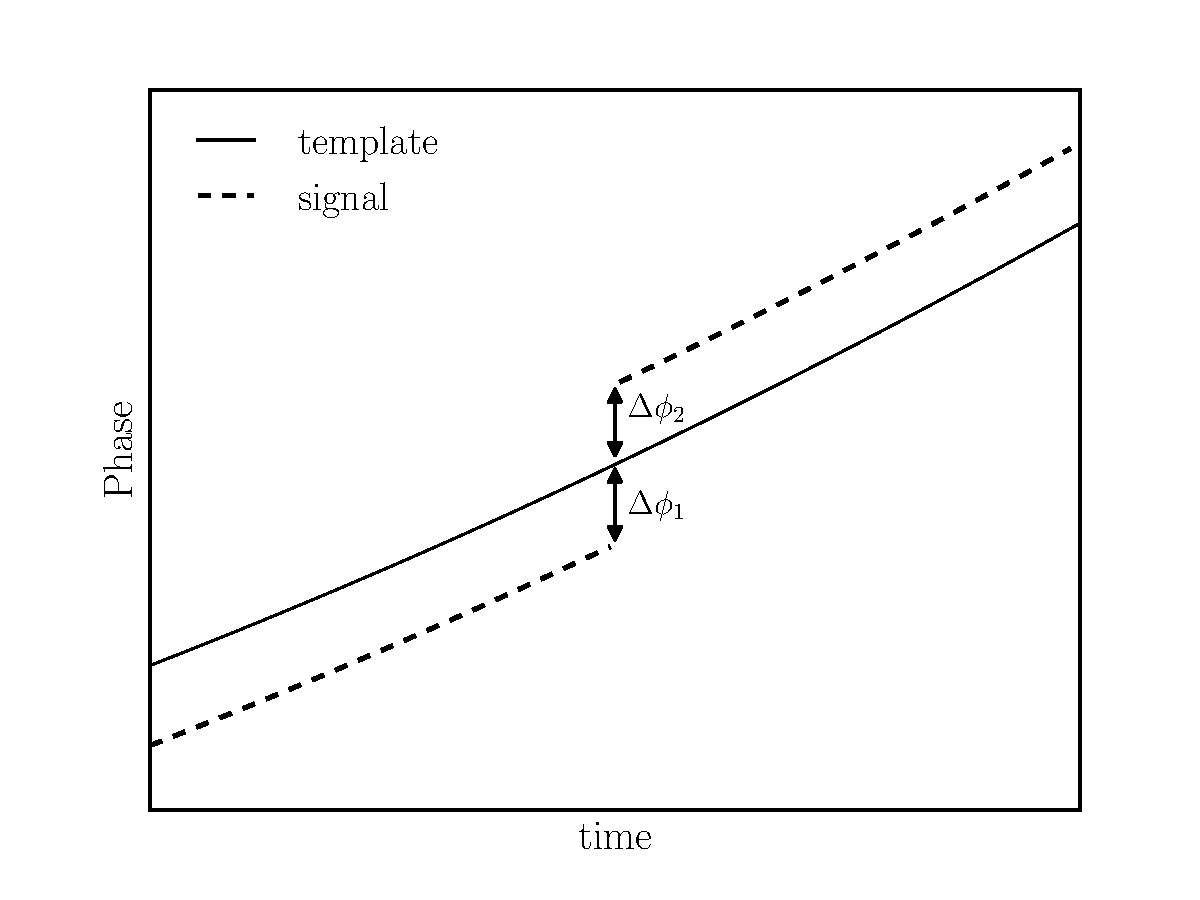
\includegraphics[width=.5\textwidth]{PhaseJump}
    \caption{Illustration of the signal and template defined in equation
        \eqref{eqn: phase offset}}
    \label{fig: PhaseJump}
\end{figure}
Parameterising by the offset with respect to the template $\bl_{0}$ for some
arbitrary template and phase jump, we write the phase deviations in the two
subdomains as
\begin{equation}
 \Delta\Phi(t) = \left\{
\begin{array}{cr}
\Delta \phi_{1}& \; 0 < t < T/2 \\
\Delta \phi_{2} & \;  T/2 < t < T
\end{array}.
\right.
\label{eqn: phase offset}
\end{equation}

To compute the matched filtering amplitude given in Eqn.~\eqref{eqn: matched
filtering amplitude}, we can factorise the integral using the additivity of
integration on intervals into two integrations
\begin{eqnarray}
X & = &\frac{1}{T } \int_{0}^{T}e^{i\Delta\Phi(t)} dt\\
 & = &\frac{1}{T }\left(\int_{0}^{T /2}e^{i\Delta\phi_{1}} dt  +
\int_{T/2}^{T} e^{i\Delta\phi_{2}}dt\right)\\
& = & \frac{1}{2}\left(e^{i\Delta\phi_{1}} + e^{i\Delta\phi_{2}}\right).
\end{eqnarray}
Because our choice in splitting up the integral exactly matches the sub-domans
defined in Eqn.~\eqref{eqn: phase offset}, and in each sub-domain $\Delta\Phi(t)$
is constant, we can compute the integrals.
The absolute square value of the matched filtering amplitude is then
\begin{eqnarray}
|X|^{2}& = &\frac{1}{4}\left(e^{i\Delta\phi_{1}} + e^{i\Delta\phi_{2}}\right) \left(e^{-i\Delta\phi_{1}} + e^{-i\Delta\phi_{2}}\right)\\
& = &\frac{1}{4} \left(2 + e^{i(\Delta\phi_{1} - \Delta \phi_{2})} +  e^{-i(\Delta\phi_{1} - \Delta_{\phi_{2}})} \right) \\
& = &\frac{1}{2}\left(1 + \cos(\Delta\phi_{1} - \Delta\phi_{2})\right).
\end{eqnarray}
Finally, the mismatch can be calculated from equation \eqref{eqn: full mismatch}.
\begin{equation}
\mu = \frac{1}{2}\left(1 - \cos(\Delta\phi_{1} - \Delta\phi_{2})\right).
\label{eqn: two segment phase mismatch}
\end{equation}

From this result we learn that it is not the phase difference with respect to
each of the Taylor expansion ($\Delta\phi_1$ or $\Delta\phi_2$) which is
important, but the total phase jump at their interface. For $\Delta \phi_{1} =
\Delta \phi_{2}$ the mismatch vanishes, this recovering the case of a single
Taylor expansion signal with an arbitary overall phase offset which always has
zero mismatch. This result can be used to calculate the mismatch due to a glitch,
if the glitch is purely in the phase; in reality we know that glitches are
discontinuities in the frequency and spin-down rate which will be considered in
Chapter~\ref{sec: glitches in cgw}.

%\paragraph{Comparing with an exact numerical result}
%\meta{Greg: potentially cut this} We can verify equation
%\eqref{eqn: two segment phase mismatch} by comparing with the results of a
%exact numerical calculation of the mismatch. This involves defining the signal
%such that it describes two segments with a phase offset, then `injecting' and
%recovering the signal using \texttt{LALApps} software. We do this in the
%absence of noise and compute the mismatch against a perfectly matched signal.
%The signal comprises two adjacent transient windows of fixed duration. We set
%the phase offset in the first segment to zero and subject the second segment to
%a phase jump $\Delta \phi$, therefore
%\begin{align}
%    \Delta \phi_{1} &= 0 &  \textrm{ and } && \Delta \phi_{2} =& \Delta\phi.
%\end{align}
%Varying $\Delta\phi$ we plot the exact numerical result along with the
%prediction of equation~\eqref{eqn: two segment phase mismatch} in
%Fig.~\ref{fig: two plot}
%\begin{figure}
%\centering
%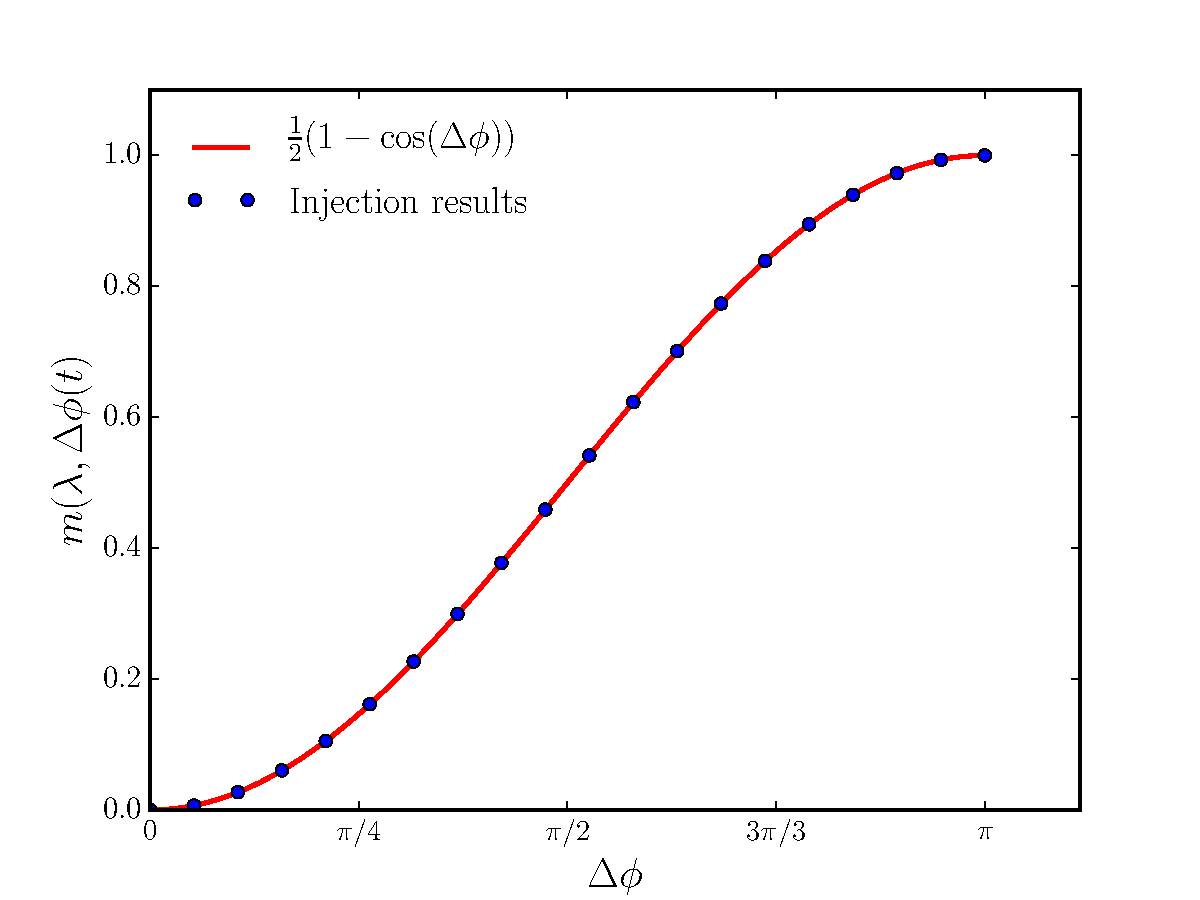
\includegraphics[width=0.65\textwidth]{Exact_analytic_phase_two_segments}
%\caption{Plot of the theoretical prediction of equation~\eqref{eqn: two segment
%phase mismatch} given a time dependent phase offset as in equation\eqref{eqn:
%phase offset}. This is compared  with a signal injection and recovery
%using \texttt{LALapps} software.}
%\label{fig: two plot}
%\end{figure}

\subsection{N subdomains with phase discontinuity's}
We can further generalise Eqn.~\eqref{eqn: two segment phase mismatch} by
letting the signal be comprised of $N$ equal duration subdomains with a phase discontinuity
$\Delta\phi_i$ for the $i^{th}$ subdomain.
Then, the matched filtering amplitude can be written
\begin{eqnarray}
X & = & \frac{1}{T}\left(\int_{0}^{t_{1}}e^{i\Delta\phi_{1}} dt +
\int_{t_{1}}^{t_{2}}e^{i\Delta\phi_{2}} dt + \dots +
\int_{t_{N-1}}^{t_{N}}e^{i\Delta\phi_{N}} dt \right) \\
& = &  \frac{1}{T}\left(\frac{T}{N}e^{i\Delta\phi_{1}} +
\frac{T}{N}e^{i\Delta\phi_{2}} + \dots + \frac{T}{N}e^{i\Delta\phi_{n}} \right)\\
& = & \frac{1}{N} \sum_{i=1}^{N}e^{i\Delta \phi_{i}}.
\end{eqnarray}
Squaring the matched filtering amplitude and simplifying
\begin{eqnarray}
|X|^{2} & = &  \frac{1}{N^{2}} \left(\sum_{i=1}^{N}e^{i\Delta \phi_{i}}\right)\left(\sum_{j=1}^{N}e^{-i\Delta \phi_{j}}\right) \\
|X|^{2} & = &  \frac{1}{N^{2}} \sum_{i=1}^{N}e^{i\Delta \phi_{i}}\left(\sum_{j=1}^{N}e^{-i\Delta \phi_{j}}\right) \\
& = & \frac{1}{N^{2}} \sum_{i=1}^{N}e^{i\Delta \phi_{i}}\left(e^{-i\Delta \phi_{i}} +  \sum_{\substack{j=1 \\j\ne i}}^{N}e^{-i\Delta \phi_{j}}\right) \\
& = & \frac{1}{N^{2}} \left(\sum_{i=1}^{N}1 +   \sum_{i=1}^{N}\sum_{\substack{j=1 \\j\ne i}}^{N}e^{i(\Delta\phi_{i}-\Delta \phi_{j})}\right) \\
& = & \frac{1}{N^{2}} \left(N +   \sum_{i=1}^{N}\sum_{\substack{j=1 \\j\ne i}}^{N}\cos(\Delta\phi_{i} - \Delta\phi_{j}) + i\sin(\Delta\phi_{i} - \Delta\phi_{j})\right).
\end{eqnarray}
In this final summation for each pair $(i,j)$ the corresponding pair $(j, i)$
will exist in the sum. This leads to a cancellation of the imaginary part and a
doubling of the real part
\begin{equation}
|X|^{2}  = \left(\frac{1}{N} + \frac{1}{N^{2}}\sum_{i=1}^{N}\sum_{\substack{j=1 \\j\ne i}}^{N} \cos(\Delta\phi_{i} - \Delta \phi_{j})\right).
\end{equation}•
Then the mismatch is given by:
\begin{equation}
\mu = 1 - \frac{1}{N} - \frac{1}{N^{2}}\sum_{i=1}^{N}\sum_{\substack{j=1 \\j\ne i}}^{N} \cos(\Delta\phi_{i} - \Delta\phi_{j}).
\label{eqn: phase mismatch}
\end{equation}

This result could be used to estimate the mismatch due to a random walk model
of timing noise where the random walk was purely in the phase (see
Sec.~\ref{sec: TN interpretations random walk models} for example)

\subsection{Oscillating phase deviations}

Timing residuals, or equivalently the phase offsets between Taylor expansions
and the real signals, are often found to have a quasi-periodic structure
\citep{Hobbs2010}. It is reasonable to ask if, because the residuals oscillate
about the origin, the loss of detection will be cancelled out. In this section
we consider such an oscillating phase deviation and show that, over many
oscillations, the mismatch is non-zero.

We model a small sinusoidal phase offset by a trigonometric function
\begin{equation}
\Delta \Phi(t) = \varepsilon \cos(\omega t),
\end{equation}•
where $\varepsilon$ is the amplitude of variatinos and $\omega$ is the angular
frequency of the oscillations. If we assume that the variations are small
$\varepsilon \ll 1$, we can Taylor expandthe exponential phase offset in
the matched filtering amplitude
\begin{equation}
X = \frac{1}{T}\int_{T}
1 + i \epsilon \cos{\left (\omega t \right )}
- \frac{\epsilon^{2}}{2} \cos^{2}{\left (\omega t \right )}
- \frac{i \epsilon^{3}}{6} \cos^{3}{\left (\omega t \right )}
dt
+ \mathcal{O}\left(\epsilon^{4}\right).
\end{equation}
Inserting this into equation~\eqref{eqn: full mismatch} and computing the
mismatch we find
\begin{equation}
\mu = \varepsilon^{2} \left(\frac{1}{2}
+ \frac{\sin{\left (2 T \omega \right )}}{4 T \omega}
+ \frac{\sin^{2}{\left (T \omega \right )}}{T^{2} \omega^{2}} \right)
+ \mathcal{O}\left(\epsilon^{4}\right).
\label{eqn: Oscillating mismatch}
\end{equation}
In the limit $T \rightarrow \infty$ this tends to $\varepsilon^{2}/2$. Before
this, the mismatch oscillates around this value over observation times similar
to the oscillation period; this is shown in figure \ref{fig:
OscillatoryPhaseMismatch}.
\begin{figure}[ht]
\centering
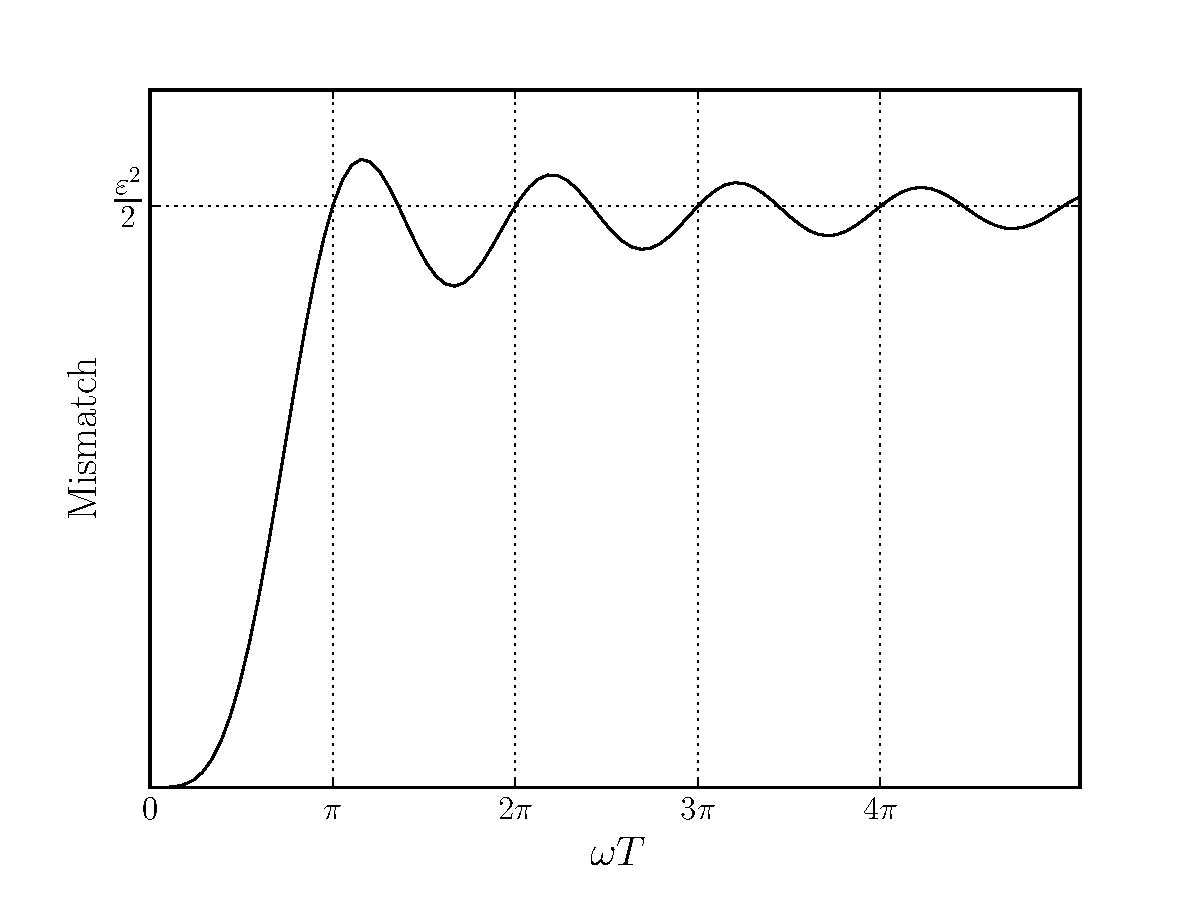
\includegraphics[width=.6\textwidth]{OscillatoryPhaseMismatch}
\caption{Plot demonstrating the behaviour of equation
         \eqref{eqn: Oscillating mismatch}, the mismatch for an oscillating
         phase offset.}
\label{fig: OscillatoryPhaseMismatch}
\end{figure}

This simple model demonstrates that if the signal and template are on average
coherent, but the phase residual between them oscillates about the mean, then
over several cycles the mismatch will approach a constant value dependent on
the maximum amplitude of the residuals.  For a quasi-periodic signal the same
overall picture will emerge with the size of the mismatch dependent on the mean
average size of oscillations in the residual.

\biblio


\end{document}
